\documentclass[journal]{IEEEtran}
\usepackage{graphicx}
\usepackage[hidelinks]{hyperref}
\usepackage{caption}
\usepackage{array}

\captionsetup[figure]{labelfont=bf,textfont={footnotesize, it},singlelinecheck=on,justification=justified}
 
%\imageOne{sizecm}{filename}{caption}{label}
\newcommand{\imageOne}[4] {
	\begingroup
		\centering
    	\includegraphics[width=#1]{#2}
	   	\captionof{figure}{#3}\label{fig:#4}
	\endgroup
}

%\imageTwo{sizecm}{filename}{caption}{label}
\newcommand{\imageTwo}[4] {
	\begin{figure*}
		\centering
		\includegraphics[height=#1]{#2}
		\captionof{figure}{#3}\label{fig:#4}
	\end{figure*}
}

% correct bad hyphenation here
%\hyphenation{op-tical net-works semi-conduc-tor}

\begin{document}

\title{Dynamic Core Processors}

\author{Kyle Daruwalla, David McNeil, and Ben Schmidt \\ \IEEEmembership{Rose-Hulman Institute of Technology}}% <-this % stops a space

% \markboth{Journal of \LaTeX\ Class Files,~Vol.~6, No.~1, January~2007}%
% {Shell \MakeLowercase{\textit{et al.}}: Bare Demo of IEEEtran.cls for Journals}

\maketitle

\begin{abstract}
As both general purpose, desktop-grade processors and embedded processors mature, the distinguishing gap between them continues to diminish. Out of this narrowing market, a need for a versatile, low-power core emerges. Multicore embedded processors are just over the horizon. Dynamic core processors attempt harness these low-power cores to maximize both parallel throughput and minimize serial latency.
\end{abstract}

\begin{IEEEkeywords}
IEEEtran, journal, \LaTeX, paper, template.
\end{IEEEkeywords}


\section{Introduction and Motivation}
Mobile computing devices have grown to require processors that can support a dynamic workload. The typical serial tasks such as voice compression, speech transcoding (for communications), and image compression must perform well. However, newer mobile devices need to render complex graphics and run advanced background scheduling, all while maintaining serial performance and power. The obvious answer might be GPUs, but they are known to be power-hungry chips. Ideally, if most of the serial and parallel tasks could be performed on a single chip, the GPU would only need to be used to perform high TLP tasks like displaying graphics. A smaller GPU workload means a lower power GPU. Thus, power consumption can be kept minimal, while performance gains are still attained.

Dynamic core processors attempt solve precisely these issues. By adding an interconnection network, some additional hardware, and control logic, the symmetric multicore embedded processors can be reconfigured into a modern, super-scaler, out-of-order processor. Thus, by identifying serial and parallel program sections, the processor can be dynamically changed to perform efficiently.

Obviously, creating such a processor, though possible, is not a trivial task. So, we attempt to analyze the theoretical performance gains of a dynamic core as described above. The following work will show whether a dynamic core processor performs better than a symmetric multicore processor and a modern, super-scalar, out-of-order processor. Furthermore, for a fixed length program, we determine how often the program must switch from serial to parallel processing before a dynamic core processor realizes performance gains. Finally, we determine the maximum number of cores in a dynamic processor before critical path length negatively impacts serial performance.

\imageOne{7cm}{../images/performance.png}{THIS IS JUST AN EXAMPLE IMAGE FROM ANOTHER PAPER Performance and power requirements of 3G wireless. Theoretical performance and power statistics of SODA, other DSPs, and general-purpose processors \cite{gem5}.}{performance}

testing images Fig. \ref{fig:performance}

\imageTwo{8cm}{../images/soda.png}{THIS IS JUST AN EXAMPLE IMAGE FROM ANOTHER PAPER The SODA Architecture \cite{gem5}}{soda}


\section{Prior Work}
Summarize relevant related work with appropriate citations.

\blindtext


\section{Methodology}
\subsection{Models}
In order to simulate a dynamic core processor without actually implementing one, the team identified two basic models - an baseline symmetric core and a modern, out-of-order core. By combining multiple baseline cores into a single multiprocessor, we could create a parallel model (i.e. a processor biased towards parallel programs). The single modern, out-of-order core makes our serial model (i.e. a processor biased towards serial programs). Thus, the third model in our study, the dynamic model, is a combination of the serial and parallel models.

Based on this methodology, we needed a simulator capable of switching between CPU types. Previous work in this area had been done using the gem5 simulator. Capable of switching between CPU types, gem5 was an ideal choice.

\subsection{Tools}
The gem5 simulator \cite{gem5} is a combination of M5, a simulation framework with support for multiple ISAs and CPU models, and GEMS, a memory simulation system in two parts - Ruby and Opal. As a result, gem5 is a robust simulator with support for five ISAs, ARM, ALPHA, MIPS, Power, SPARC, and x86, and four CPU models:

\begin{itemize}
	\item AtomicSimple is a minimal single IPC CPU model
	\item TimingSimple is similar to AtomicSimple but also simulates the timing of memory references,
	\item InOrder is a pipelined, in-order CPU
	\item O3 is a pipelined, out-of-order CPU model
\end{itemize}

gem5 has two modes of operation - system emulation mode and full system mode. System emulation mode does not model the OS or peripheral devices but solely simulates the specified benchmark. Full system mode, on the other hand, uses an actual OS kernel and mounts a Linux disk image. Essentially, gem5 full system mode is capable of booting a full OS and presenting the user with a Linux command prompt.

Initially, gem5's many high level customizations suggested that it would be an effective simulator for a dynamic processor model. However, while gem5 may boast many impressive features, we found that many of these features are not fully supported or difficult to configure.

\begin{table}[!t]
	\renewcommand{\arraystretch}{1.9}
	\centering
	\begin{tabular}{|c|c|c|}
		\hline
		Benchmark & Description & Parameters\\
		\hline
		ocean & placeholder & placeholder\\
		\hline
		fft & placeholder & placeholder\\
		\hline
		lu & placeholder & placeholder\\
		\hline
		radix & placeholder & placeholder\\
		\hline
	\end{tabular}
	\caption{The SPLASH-2 benchmarks used}
	\label{tab:splash2_benchmarks}
\end{table}

\begin{table}[!t]
	\renewcommand{\arraystretch}{1.9}
	\centering
	\begin{tabular}{|c|c|c|}
		\hline
		Benchmark & Description & Parameters\\
		\hline
		jpeg & placeholder & placeholder\\
		\hline
		epic & placeholder & placeholder\\
		\hline
		gsm & placeholder & placeholder\\
		\hline
		adpcm & placeholder & placeholder\\
		\hline
	\end{tabular}
	\caption{The MediaBench II benchmarks used}
	\label{tab:mb2_benchmarks}
\end{table}

For simulation of a dynamic processor, we needed two types of benchmarks. One which would be representative of highly parallelized workloads and one reflecting serial execution. The parallel benchmark we used was SPLASH-2 \cite{splash2}. SPLASH-2 is a suite of benchmarks intended to evaluate the performance of multiprocessor systems. For a serial benchmark suite, we chose to use MediaBench II \cite{mb2}. A suite of compression and decompression multimedia algorithms. The programs selected from each benchmark were intended to accurately reflect typical mobile device usage. Tables \ref{tab:splash2_benchmarks} and \ref{tab:mb2_benchmarks} detail the exact benchmarks used.

\subsection{Procedure}
When we initially began the project we planned on using gem5 SE mode for simplicity. However, due to the parallel nature of SPLASH-2 a multi-threading library is required. Because SE mode does not emulate a full operating system, there was no OS-level threading library such as pthreads. As a result, we finally decided to use full system mode. This provided us with access to Linux's full threading library allowing us to simulate the multi-threaded applications. Using full system mode had the additional benefit of providing extremely accurate results because the benchmarks are actually running in a Linux operating system, similar to our application space.

At this point, it was necessary to determine what CPU types and ISAs would be tested in order to simulate a dynamic processor. We initially planned on using either x86 or ARM as the underlying ISA. However, we soon found that only AtomicSimple CPU model was supported by gem5 full system mode for these ISAs. gem5 provides much more complete support for the ALPHA ISA. ALPHA is a 64-bit RISC ISA representative of a simply architected general processor. Using this ISA as our building block we were able to develop benchmarks to represent a serial and a parallel machine. Our serial system used the O3 CPU model to simulate a modern out of order processor. Our parallel system was comprised multiple TimingSimple CPU models. Originally, we had intended to use the InOrder model, however it was not available. Even though the TimingSimple CPU type was not a standard in-order pipeline, an array of the single cycle cores out performed the out-of-order processor on most parallel benchmarks. Thus, we felt the loss in accuracy was negligible.

In order to efficiently run tests, we developed scripts to boot a Linux kernel in FS mode and run through each of our benchmarks. At the completion of each benchmark the timing statistics would be written out to file. A script was then developed capable of parsing the output file and produce a CSV file containing the statistics for each benchmark. The Linux boot process became an advantage in our setup. Spanning 2.4 trillion instructions, we could be confident that all our caches would be warmed up after the boot process was complete. Furthermore, gem5's built-in stats-dump tool allowed us to run serial and parallel benchmarks one after the other without shutting the system down. This meant that the cache state before each benchmark was exactly the cache state at the end of the previous benchmark; thus, the initial cache miss latencies were embedded into our timing results.

Once we had the timing results for the serial and parallel models, we synthesized the results together to get the timing performance for a dynamic core. Of course, there is some latency associated with switching from a serial configuration to a dynamic configuration. Though we did not implement a dynamic core, we did theorize potential methods for a datapath. In particular, we were drawn to the idea of using muxes to run external inputs into the execution units of several cores. Based on this, it seemed appropriate that an advanced interconnect network would be required. Most multicore and SoC devices use a crossbar network, but the crossbar is hardly scalable. Instead, many bleed-edge devices use network-on-chip (NoC) structures that are based off of crossbar interconnects, but optimized for scalability and power dissapation. Thus, we selected a switching latency of 0.991 ns based on research in the field of NoCs \cite{lee}.

Furthermore, in order to study the problems surrounding a dynamic processor, we tackled two optimization issues. First, we chose a single serial program and a single parallel program to make up a single ``chunk'' of mixed code. We then look run time for 512 chunks put together. Then, the size of the serial and parallel portion in a chunk were doubled, so that each chunk is twice as large as it was before. However, we now only use 256 chunks in the test, so that the overall number of instructions remains constant. Repeating this process of doubling the size of a serial chunk and a parllel chunk while halving the number of chunks in the program, we are able to get results for the number of switches for maximum performance between serial and parallel portions within a fixed code segment. Secondly, we recognized that as the number of cores in the parallel model increases, the critical path of the serial model increases. Thus, the frequency should scale down for the serial model. Based on simple geometry (Pythagorean's theorem), we assume that the frequency will scale on the order of $1 / \sqrt{n}$. Thus, we obtained results for the serial model with scaled frequencies to see if there is a drop-off in performance.

\section{Results}
Provide and justify any quantitative results, preferably using graphs
and/or tables. 

\section{Conclusion and Future Work}
Overall, the results of the study were promising. A dynamic core performs better than both a symmetric multicore machine, as well as a modern, out-of-order processor. We identified an approximate power overhead for a dynamic core; we argue that this overhead is minimal compared to the total power consumption, and that a dynamic core receives 1.2x speedup with a small loss in power efficiency. Furthermore, we identified that fine grained context switching between serial and parallel workloads degrades performance on a dynamic core. Finally, the study noted that there is peak performance gain for a dynamic core as the number of baseline cores is scaled. This was due to an increased critical path for the serial model.

Even though the dynamic core did not perform better than a dual core modern, out-of-order processor, we were able to identify areas for improvement. First, creative critical path routing will significantly help the performance of a dynamic core. Secondly, coarse grained context switching will maximize performance. As always, it was clear that Amdahl's Law still holds true, and both serial and parallel performance need to be patiently maximized to gain better overall performance.

The critical path issue lends itself nicely to 3D stacking technologies. Take, for example, a baseline core that is serving as a functional unit for the serial model. This core will receive data from another baseline core's register file. Using 3D stacking, the two cores could be placed on top of each other, so that the path from the register file of one core to the execution unit of another is small.

In addition to analyzing the performance gains of 3D stacking technologies, the study would be best served by a re-analysis of the serial and parallel models. For our theoretical study, the ALPHA ISA was sufficient, but a more accurate serial model would be an out-of-order x86 core, and a more accurate parallel model would be a multicore ARMv7 machine.

Keeping this future work in mind, there is still plenty of room for the dynamic core model to grow. Theoretical research such as ours needs to be done, as well as implementation research to get more accurate latency times. Dynamic cores alone will not help mobile device manufacturers, but a combination of dynamic cores with other technologies could prove to be an effictive speedup with minimal loss in power efficiency.

\section{Statement of Work}
\begin{figure*}
    \centering
    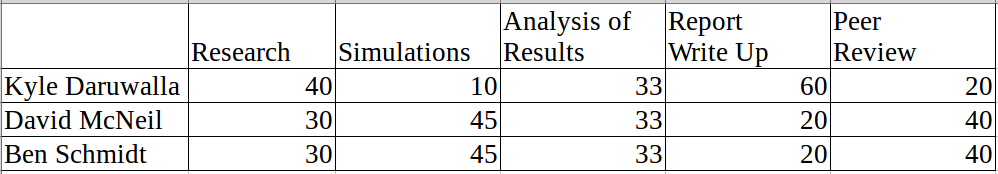
\includegraphics[scale=0.4]{../images/statement_of_work.png}
    \caption{Contributions of individual team members}
    \label{fig:statement_of_work}
\end{figure*}
See Figure \ref{fig:statement_of_work} \\
Signed by: Kyle Daruwalla, David McNeil, and Ben Schmidt

%\appendices
%\section{Proof of the First Zonklar Equation}
%Some text for the appendix.

% use section* for acknowledgement
\section*{Acknowledgment}
The authors would like to thank...

\begin{thebibliography}{1}
\bibitem{gem5}
  N. Binkert, B. Beckmann, G. Black, S. Reinhardt, A. Saidi, A. Basu, J Hestness, D. Hower, T. Krishna, S. Sardashti, R. Sen, K. Sewell, M. Shoaib, N. Vaish, M. Hill, D. Wood.
  ``The gem5 Simulator,'' 
  Available: \url{http://research.cs.wisc.edu/multifacet/papers/can11_gem5.pdf}

\bibitem{splash2}
  Not sure how to site this.
  Available: \url{http://www.capsl.udel.edu/splash/index.html} 
  
\bibitem{mb2}
  Not sure how to site this.
  Available: \url{http://euler.slu.edu/~fritts/mediabench/} 

\end{thebibliography}

%\begin{IEEEbiography}[{
\includegraphics[width=1in,height=1.25in,clip,keepaspectratio]{picture}}]{John Doe}
%\end{IEEEbiography}


\end{document}


